\documentclass{beamer}
\usepackage[T1]{fontenc}
\usepackage{fancyvrb}
\usepackage{minted}

\title{Ray Marching}
\author{John Owen}
\date{}

\newcommand\imageframe[1]{
    \begin{frame}[plain]
        \includegraphics[keepaspectratio=true,width=1\paperwidth]{../img/#1}
    \end{frame}
}

\begin{document}

\frame{\titlepage}

\imageframe{raymarch1.png}
\imageframe{raymarch2.png}
\imageframe{raymarch3.png}
\imageframe{raymarch4.png}
\imageframe{raymarch5.png}
\imageframe{raymarch6.png}
\imageframe{raymarch7.png}
\imageframe{raymarch8.png}
\imageframe{raymarch9.png}
\imageframe{raymarch10.png}

\begin{frame}[fragile]
    \frametitle{Distance functions}
    \begin{columns}
        \column{.5\textwidth}
        Sphere:
    \begin{minted}[fontsize=\footnotesize]{glsl}
float sdfSphere(vec3 p, float radius) {
  return length(p) - radius;
}
    \end{minted}
        \column{.5\textwidth}
        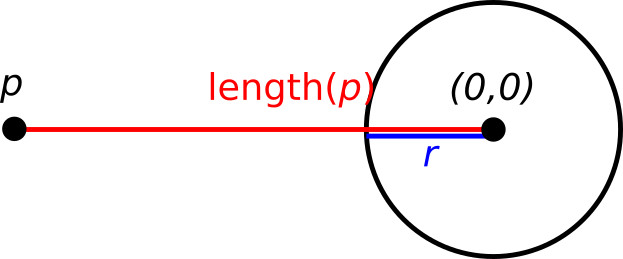
\includegraphics[keepaspectratio=true,width=\textwidth]{../img/looking-outside-circle.png}
    \end{columns}
\end{frame}

\begin{frame}[fragile]
    \frametitle{Distance functions}
    \begin{minted}[fontsize=\small]{glsl}
float dfBox(vec3 p, vec3 size) {
  return length(max(abs(p) - size / 2., 0.));
}

float sdfCylinder(vec3 p, float radius, float height) {
  vec2 h = vec2(radius, height / 2.);
  vec2 d = abs(vec2(length(p.yz), p.x)) - h;
  return min(max(d.x, d.y), 0.0) + length(max(d, 0.0));
}

float sdfPlane(vec3 p, vec3 normal, float distance) {
  return dot(p, normal) + distance;
}
    \end{minted}
\end{frame}


\begin{frame}[fragile]
    \frametitle{Sphere Tracing Algorithm}
    \begin{minted}[fontsize=\footnotesize]{glsl}
void main() {
  gl_FragColor = (0.7, 0.8, 0.9, 1.) // Start with a sky color
  vec3 ro = vec3(1., 0., 5.); // Ray origin
  vec3 rd = rayDirection();
  float t = 0.; // How far we've travelled along the ray so far
  for (int i = 0; i < 1000; i++) { // March 1000 times
    vec3 p = ro + rd * t; // The point along the ray we are at
    float d = sdfSphere(p, 2.); // Distance of p to sphere of radius 2
    t += d; // Move forward along the ray
    if (d < 0.001) { // If p close to boundary sphere
      // Compute the lighting, shadows, etc
      gl_FragColor = computeShadingForPoint(p);
      break;
    }
    if (t > 100) // If the ray missed the sphere completely
      break;
  }
}
    \end{minted}
\end{frame}

\begin{frame}[fragile]
    \frametitle{Translation}
    \begin{columns}
        \column{.5\textwidth}
        We can translate a shape by shifting the \texttt{p} value:

        \begin{minted}[fontsize=\footnotesize]{glsl}
// A sphere of radius 2 at (-1,1,0).
float sdfScene(vec3 p) {
    p -= vec3(-1., 1., 0.);
    return sdfSphere(p, 2.);
}
        \end{minted}
        \column{.5\textwidth}
        (image)
    \end{columns}
\end{frame}

\end{document}
